\documentclass[a4paper]{article}
%\usepackage{enumitem, amsmath, gensymb, graphicx, caption, amssymb, geometry, fancyhdr, arydshln, adjustbox}
\usepackage{enumitem, amsmath, geometry, fancyhdr, arydshln, amssymb, float, graphicx}

\geometry{left=1in, right=1in, top=1in, bottom=1in}
\pagestyle{fancy}

\newcommand{\myName}{\textbf{Shantanu Ghodgaonkar}\\\textit{Univ ID}: N11344563\\\textit{Net ID}: sng8399\\\textit{Ph.No.}: +1 (929) 922-0614}
\newlist{qalist}{description}{1}
\setlist[qalist]{style=unboxed,leftmargin=0.5cm,labelwidth=2.5cm}


\title{Homework 5 Answers : ROB-GY 6003}
\author{\myName}
\date{\today}

\fancyhead{} % Clear existing header settings 
\fancyhead[L]{\today}
\fancyhead[R]{N11344563}


\begin{document}
	
	\begin{titlepage}
	    \centering
	    \vspace{2cm}
	    \Huge\textbf{Foundations of Robotics \\ ROB-GY 6003 \\ Homework 5 Answers}
	    \vspace{1cm}
	    \\ \Large \today
	    \vfill 
	    \Large \myName
	\end{titlepage}
	
	\begin{qalist}			
		\item[Question: 6.15] \setcounter{equation}{0} %28
		\item[Answer:] Given in below Fig~\ref{fig:q6_15} is the manipulator in question -
			\begin{figure}[H]			
				\vspace{0.5cm}
				\centering
				\fbox{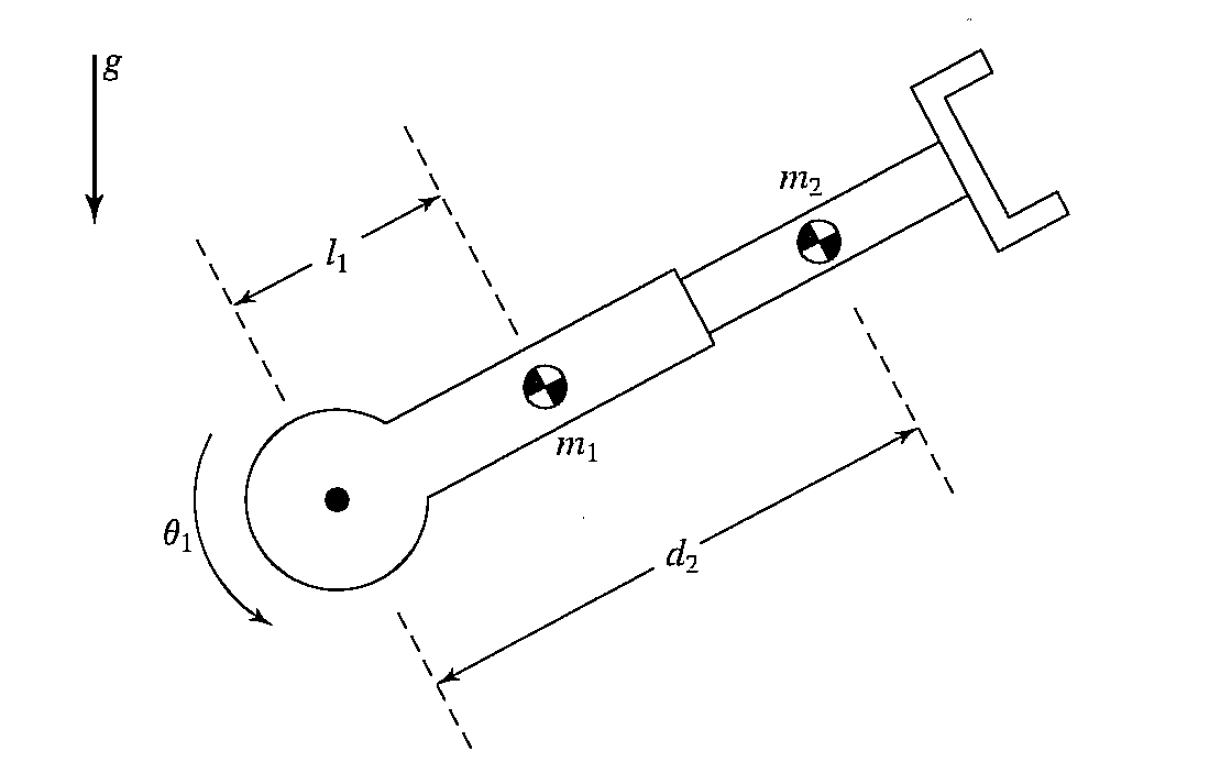
\includegraphics[width=0.75\textwidth]{q6_15.png}}
				\caption{The RP manipulator} 
				\label{fig:q6_15}
				\vspace{0.5cm}
			\end{figure}
			The links of the manipulator have the intertia tensors,
			\begin{align}
				{}^{{C}_{1}}{I}_{1} &= \begin{bmatrix} {I}_{xx1} & 0 & 0 \\ 0 & {I}_{yy1} & 0 \\ 0 & 0 & {I}_{zz1} \end{bmatrix} \notag \\
				{}^{{C}_{2}}{I}_{2} &= \begin{bmatrix} {I}_{xx2} & 0 & 0 \\ 0 & {I}_{yy2} & 0 \\ 0 & 0 & {I}_{zz2} \end{bmatrix}
			\end{align}
			
			The links have a mass of ${m}_{1}$ and ${m}_{2}$ respectively. The center of mass of link 1 is located as distance ${l}_{1}$ from joint-1 axis and that of link 2 is at the variable distance ${d}_{2}$, from the joint-1 axis.
			
			We know that, 
			\begin{equation} \label{eq:KEoM}
				{k}_{i} = \frac{1}{2} {m}_{i} {v}^{T}_{{C}_{i}} {v}_{{C}_{i}} + \frac{1}{2} {}^{i} {\omega}^{T}_{i} {}^{{C}_{i}}{I}_{i} {}^{i}{\omega}_{i}
			\end{equation}
			Using above ${Eq}^{n}~(\ref{eq:KEoM})$ we write the kinetic energy for link 1 \& 2 $\rightarrow$
			\begin{align}
				\label{eq:KEoL1}{k}_{1} &= \frac{1}{2} {m}_{1} {l}^{2}_{1} \dot{{\theta}^{2}_{1}} + \frac{1}{2}  {I}_{zz1} \dot{{\theta}^{2}_{1}} \\
				\label{eq:KEoL2}{k}_{2} &= \frac{1}{2} {m}_{2} ({d}^{2}_{2} \dot{{\theta}^{2}_{1}} + \dot{{d}^{2}_{2}}) + \frac{1}{2}  {I}_{zz2} \dot{{\theta}^{2}_{1}} \\ 
				\label{eq:KETot} \Rightarrow k(\Theta, \dot{\Theta}) &= \frac{1}{2} ({m}_{1}{l}^{2}_{1} + {I}_{zz1} + {I}_{zz2} + {m}_{2} {d}^{2}_{2}) \dot{{\theta}^{2}_{1}} + \frac{1}{2} {m}_{2} \dot{{d}^{2}_{2}}
			\end{align}
			
			We also know that, 
			\begin{equation}\label{eq:PEoL}
				{u}_{i} = -{m}_{i} {}^{0}{g}^{T} {}^{0}{P}_{{C}_{i}} + {u}_{{ref}_{i}}
			\end{equation}
			
			Using above  ${Eq}^{n}~(\ref{eq:PEoL})$ we write the potential energy for link 1 \& 2 $\rightarrow$
			\begin{align}
				\label{eq:PEoL1} {u}_{1} &= {m}_{1} {l}_{1} g \sin({\theta}_{1}) + {m}_{1} {l}_{1} g \\
				\label{eq:PEoL2} {u}_{2} &= {m}_{2} g {d}_{2} \sin({\theta}_{1}) + {m}_{2} g {d}_{2max} \\
				\label{eq:PETot} \Rightarrow  u(\Theta) &= g ({m}_{1} {l}_{1} + {m}_{2} {d}_{2} ) \sin({\theta}_{1}) + {m}_{1} {l}_{1} g + {m}_{2} g {d}_{2max}
			\end{align}
			
			Taking partial derivatives, 
			\begin{align}
				\label{eq:PD1}\frac{\partial k}{\partial \dot{\Theta}} &= \begin{bmatrix} ({m}_{1} {l}^{2}_{1} + {I}_{zz1} + {I}_{zz2} + {m}_{2}{d}^{2}_{2})\dot{{\theta}_{1}} \\ {m}_{2} {d}_{2} \end{bmatrix} \\ 
				\label{eq:PD2} \frac{\partial k}{\partial \Theta} &= \begin{bmatrix} 0 \\ {m}_{2}{d}_{2}{\dot{\theta}}^{2}_{1} \end{bmatrix} \\
				\label{eq:PD3} \frac{\partial u}{\partial \Theta} &= \begin{bmatrix}g({m}_{1} {l}_{1} + {m}_{2}{d}_{2}) \cos({\theta}_{1}) \\ g{m}_{2} \sin ({\theta}_{1})\end{bmatrix}
			\end{align}
			We know that the equation for $n \times 1$ vector of actuator torques is given by, 
			\begin{equation}\label{eq:ActTorq}
				\frac{d}{dt} \frac{\partial k}{\partial \dot{\Theta}} - \frac{\partial k}{\partial \Theta} + \frac{\partial u}{\partial \Theta} = \tau
			\end{equation}
			
			Substituting  ${Eq}^{n}~(\ref{eq:PD1}),~(\ref{eq:PD2})~\&~(\ref{eq:PD3})$ in   ${Eq}^{n}~(\ref{eq:ActTorq})$, 
			\begin{align}
				\label{eq:Torq1} {\tau}_{1} &= ({m}_{1} {l}^{2}_{1} + {I}_{zz1} + {I}_{zz2} + {m}_{2}{d}^{2}_{2})\ddot{{\theta}_{1}} + 2{m}_{2} {d}_{2}\dot{{\theta}_{1}}\dot{{d}_{2}} + ({m}_{1} {l}_{1} + {m}_{2} {d}_{2} )g \cos({\theta}_{1}) \\ 
				\label{eq:Torq2} {\tau}_{2} &= {m}_{2}\ddot{{d}_{2}} - {m}_{2} {d}_{2} \dot{{\theta}^{2}_{1}} + {m}_{2} g \sin({\theta}_{1})
			\end{align}
			Finally, 
			\begin{align}
				\notag M(\Theta) &= \begin{bmatrix} ({m}_{1} {l}^{2}_{1} + {I}_{zz1} + {I}_{zz2} + {m}_{2}{d}^{2}_{2})  & 0 \\ 0 & {m}_{2}\end{bmatrix} \\ 
				\label{eq:FIN} V (\Theta, \dot{\Theta}) &= \begin{bmatrix} 2{m}_{2}{d}_{2} \dot{{\theta}_{1}}\dot{{d}_{2}} \\ -{m}_{2}{d}_{2}\dot{{\theta}^{2}_{1}}\end{bmatrix} \\ 
				\notag G(\Theta) &= \begin{bmatrix} ({m}_{1} {l}_{1} + {m}_{2}{d}_{2}) g \cos({\theta}_{1}) \\ {m}_{2}g\sin({\theta}_{1})\end{bmatrix}
			\end{align}
		\item[Question: 6.16] \setcounter{equation}{0} %25
		\item[Answer:] Upon inspection, 
			\begin{equation}
				\tau = \begin{bmatrix} {f}_{1} \\ {\tau}_{2} \end{bmatrix} = M(\theta) \ddot{\theta} + V({\theta}_{1}\dot{\theta}) + G(\theta)
			\end{equation}
			
			Where, $\theta = \begin{bmatrix} {d}_{1} \\ {\theta}_{2}\end{bmatrix}$. This implies that, 
			\begin{align}
				M(\theta) &= \begin{bmatrix} {M}_{1} + {M}_{2}  & 0 \\ 0 & {I}_{zz2} \end{bmatrix} \notag \\
				V({\theta}_{1} \dot{\theta}) &= 0 \notag \\
				G(\theta) &= 0 \notag
			\end{align}
		
		\newpage
		
		\item[Question: 6.20] \setcounter{equation}{0} %28
		\item[Answer:] Given in below Fig~\ref{fig:q6_20} is the manipulator in question -
			\begin{figure}[H]			
				\vspace{0.5cm}
				\centering
				\fbox{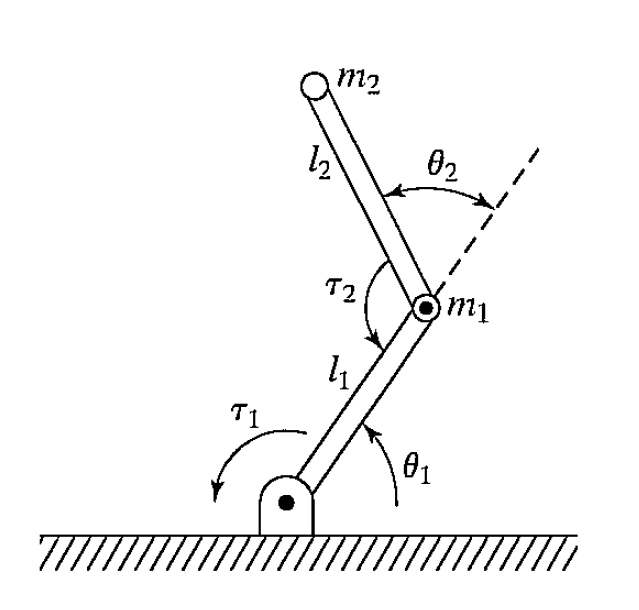
\includegraphics[width=0.75\textwidth]{q6_20.png}}
				\caption{Two-link planar manipulator with point masses at distal ends of links} 
				\label{fig:q6_20}
				\vspace{0.5cm}
			\end{figure}
			
			Because of the point-mass assumption, 
			\begin{align}
				{}^{{C}_{1}}{I}_{1} &= 0 \notag \\
				{}^{{C}_{2}}{I}_{2} &= 0
			\end{align}
			Also, as the base of the robot is not rotating, 
			\begin{align}
				{\omega}_{0} &= 0 \notag \\
				\dot{{\omega}_{0}} &= 0
			\end{align}
			We know that, 
			\begin{equation} \label{eq:KEoM}
				{k}_{i} = \frac{1}{2} {m}_{i} {v}^{T}_{{C}_{i}} {v}_{{C}_{i}} + \frac{1}{2} {}^{i} {\omega}^{T}_{i} {}^{{C}_{i}}{I}_{i} {}^{i}{\omega}_{i}
			\end{equation}
			Using above ${Eq}^{n}~(\ref{eq:KEoM})$ we write the kinetic energy for link 1 \& 2 $\rightarrow$
			\begin{align}
				\label{eq:KEoL1}{k}_{1} &= \frac{1}{2} {m}_{1} {l}^{2}_{1} \dot{{\theta}^{2}_{1}} \\
				\label{eq:KEoL2}{k}_{2} &= \frac{1}{2} {m}_{2} {l}^{2}_{2} \dot{{\theta}^{2}_{2}} \\
				\label{eq:KETot} \Rightarrow k(\Theta, \dot{\Theta}) &= \frac{1}{2} ({m}_{1}{l}^{2}_{1} \dot{{\theta}^{2}_{1}} + {m}_{2}{l}^{2}_{2} \dot{{\theta}^{2}_{2}})
			\end{align}	
				
			We also know that, 
			\begin{equation}\label{eq:PEoL}
				{u}_{i} = -{m}_{i} {}^{0}{g}^{T} {}^{0}{P}_{{C}_{i}} + {u}_{{ref}_{i}}
			\end{equation}
			
			Using above  ${Eq}^{n}~(\ref{eq:PEoL})$ we write the potential energy for link 1 \& 2 $\rightarrow$
			\begin{align}
				\label{eq:PEoL1} {u}_{1} &= {m}_{1} {l}_{1} g \sin({\theta}_{1}) + {m}_{1} {l}_{1} g \\
				\label{eq:PEoL2} {u}_{2} &= {m}_{2} {l}_{2} g\sin({\theta}_{2}) + {m}_{2} {l}_{2}g \\
				\label{eq:PETot} \Rightarrow  u(\Theta) &= g ({m}_{1} {l}_{1}\sin({\theta}_{1}) + {m}_{2} {l}_{2}\sin({\theta}_{2}) )  + {m}_{1} {l}_{1} g + {m}_{2} {l}_{2}g
			\end{align}
			We know that the equation for $n \times 1$ vector of actuator torques is given by, 
			\begin{align}
				\label{eq:ActTorq} \tau &=  \frac{d}{dt} \frac{\partial k}{\partial \dot{\Theta}} - \frac{\partial k}{\partial \Theta} + \frac{\partial u}{\partial \Theta} \\
				\Rightarrow {\tau}_{1} &= {m}_{2} {l}^{2}_{2} (\ddot{{\theta}_{1}} + \ddot{{\theta}_{2}}) + {m}_{2}{l}_{1}{l}_{2}{c}_{2}(2\ddot{{\theta}_{1}} + \ddot{{\theta}_{2}}) + ({m}_{1} + {m}_{2}){l}^{2}_{1} \ddot{{\theta}_{1}} - {m}_{2} {l}_{1} {l}_{2} {s}_{2} \dot{{\theta}^{2}_{2}} \notag \\
				&-2{m}_{2}{l}_{1}{l}_{2}{s}_{2}\dot{{\theta}_{1}}\dot{{\theta}_{2}} + {m}_{2}{l}_{2}g{c}_{12} + ({m}_{1} + {m}_{2}){l}_{1}g{c}_{1} \\ &\& \notag\\
				 {\tau}_{2} &= {m}_{2}{l}_{1}{l}_{2}{c}_{2}\ddot{{\theta}_{1}} + {m}_{2}{l}_{1}{l}_{2}{s}_{2}\dot{{\theta}^{2}_{1}} +{m}_{2}{l}_{2}g{c}_{12} + {m}_{2}{l}^{2}_{2}(\ddot{{\theta}_{1}} + \ddot{{\theta}_{2}})
			\end{align}
			
			Therefore, 
			\begin{align}
				M(\Theta) &= \begin{bmatrix} {m}_{2} + \frac{{m}_{1}}{{s}^{2}_{2}} & 0 \\ 0 & {m}_{2}\end{bmatrix} \\
				V(\Theta, \dot{\Theta}) &= \begin{bmatrix} -({m}_{2} {l}_{2} {c}_{2} + {m}_{2}{l}_{2}) \dot{{\theta}^{2}_{1}} - {m}_{2}{l}_{2}\dot{{\theta}^{2}_{2}} -(2{m}_{2}{l}_{2} + {m}_{2}{l}_{1}{c}_{2} + {m}_{1}{l}_{1}\frac{{c}_{2}}{{s}^{2}_{2}})\dot{{\theta}_{1}}\dot{{\theta}_{2}} \\  {m}_{2}{l}_{1}{s}_{2}\dot{{\theta}^{2}_{1}} + {l}_{1}{m}_{2}{s}_{2}\dot{{\theta}_{1}} \dot{{\theta}_{2}} \end{bmatrix} \\
				G(\Theta) &= \begin{bmatrix} {m}_{1}g\frac{{c}_{1}}{{s}_{2}} + {m}_{2}g{s}_{12} \\ {m}_{2}g{c}_{12} \end{bmatrix}
			\end{align}
			
	\end{qalist}
\end{document}